

\section{Introduction}\label{sec:Introduction}
Globular clusters (\acsp{GC})\acused{GC} are self-gravitating, gas-free systems of 10\(^5\) to 10\(^7\) stars which are spherically grouped with a typical size of a few parsecs and mass around $10^5$ to \unit[$10^6$]{M$_\odot$}. There are about 150 of them in the \ac{MW} \citep{1996AJ....112.1487H}. Since they are some of the oldest stellar populations in the universe (approximately \unit[13]{Gyr} old), they contain much information about the assembly history and evolution of the \ac{MW}. Formerly seen as very simple spherical and isotropic stellar systems with only one stellar population \citep{1997A&ARv...8....1M}, recent research revealed a much higher degree of complexity. \acp{GC} are now known to host multiple stellar populations that challenge our understanding of their formation (that differ in the light-elements abundances, \citealp{2015AJ....149...91P}). Moreover, \acp{GC} now also appear dynamically complex, presenting deviations from spherical symmetry, anisotropy in velocity space and significant internal rotation (see for example \citealp{2012A&A...539A..65Z,2013ApJ...772...67B,2014A&A...567A..69K}).
\par Recent attention has been devoted to the search of \acfp{IMBH} in the centre of \acp{GC}. These elusive black holes with masses of \(\unit[10^3]{\mathrm{M}_\odot} < \mathrm{M}_\bullet < \unit[10^4]{\mathrm{M}_\odot}\) could be the missing link between stellar mass black holes (\(\mathrm{M}_\bullet < \unit[100]{\mathrm{M}_\odot}\)) and super massive black holes (\acsp{SMBH}, \(\mathrm{M}_\bullet > \unit[10^5]{\mathrm{M}_\odot}\))\acused{SMBH}  (see \citealt[p.639]{2006ima..book.....C}), as they could represent the seed for the formation of \acp{SMBH}. Their search in the centre of \acp{GC} has partially been motivated by the extrapolation of the \(\mathrm{M}_\bullet-\sigma\)-relation for galaxies \citep{2000ApJ...539L...9F}, describing the relation between the mass of a central massive black hole and the velocity dispersion of its host galaxy.
\par The hunt of \acp{IMBH} in Galactic \acp{GC} has been primarily based on two methods: 
\begin{itemize}
\item[1)] detection of radio and X-ray emission due to the accretion of gas in the black hole \citep{2002MNRAS.330..232C,2008MNRAS.389..379M,2012A&A...542A..44K,2012ApJ...750L..27S}; 
\item[2)] detection of kinematic signatures in the central region of a \ac{GC} \citep{1976ApJ...209..214B,2013A&A...552A..49L}.
\end{itemize} 
The first method proved to be difficult because the feeding of a black hole with gas is highly inefficient in a gas poor environment like the one of Galactic \acp{GC}. 
\par The kinematic detection of \acp{IMBH} is usually based on the analysis of the velocity-dispersion profile in the inner few arcseconds around the crowded centre of a \ac{GC} in search for a rise of the velocity dispersion. This requires a combination of high angular resolution and high spectral resolving power. For this reason, the detection of \acp{IMBH} remains still highly challenging. 
\par Currently, there are two different kinematic methods trying to detect \acp{IMBH}: resolved kinematics of discrete stars and unresolved integrated light kinematic measurements (see, for example \citealp{2015MNRAS.453..365B}). These methods often deliver significant different results when applied to the same \ac{GC}.
\begin{figure}[htbp]
\centering
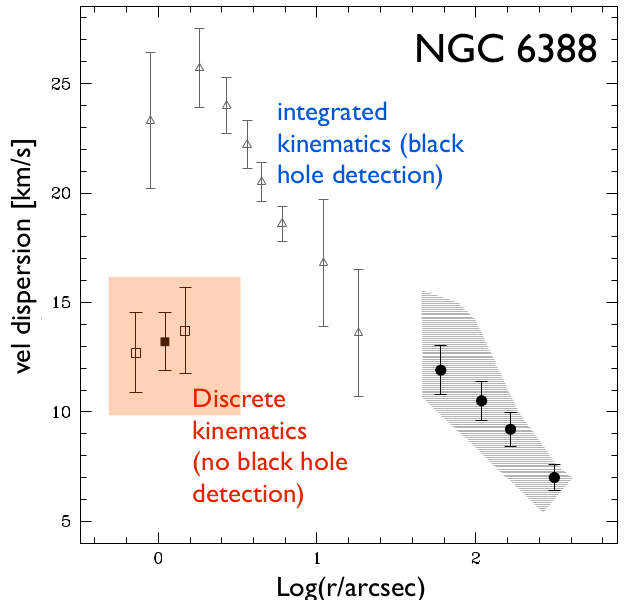
\includegraphics[width=0.5\textwidth]{Plots/Paolo_talk_plot.png}
\caption{Velocity profile of NGC 6388 derived by the two different kinematic measurements (unresolved/integrated versus resolved/discrete). We see a cusp given by the integrated kinematics method, indicative of the presence of an \ac{IMBH}, while no cusp is observed with discrete kinematics. Figure adapted from \citet{2013ApJ...769..107L}.}
\label{fig:NGC6388}
\end{figure}
As an example, Figure \ref{fig:NGC6388} shows the unresolved/integrated IFU kinematics which result in a signature of an \ac{IMBH} for NGC 6388 (cusp in the velocity dispersion profile, \citealp{2011A&A...533A..36L}) and resolved/discrete kinematics which do not yield \acp{IMBH} (no cusp in the velocity dispersion profile, \citealp{2013ApJ...769..107L}). 

\par The first proposed detected \ac{IMBH} of a \ac{GC}  using integrated light IFU kinematics was in \(\omega\) centauri \citep{2008ApJ...676.1008N} observing a rising velocity profile. Two years later, \citet{2010ApJ...710.1063V} used \ac{HST} proper motions and a different photometric centre and they could not detect the \ac{IMBH}. From then, many additional investigations were done for this \ac{GC}, unsettingly giving contradictory results. For example, using the method of detection of X-ray emission there was no \ac{IMBH} found \citep{2015A&A...581A...1L}.
\par Given these controversial results that prevent us from drawing definite conclusions on the existence of \acp{IMBH} in Galactic \acp{GC}, we propose to introduce a new approach to analyse the effects of an \ac{IMBH} to the central kinematic of a \ac{GC}. Our method consists in going beyond the traditional phase space analysis (i.e., analysis of velocity dispersion profiles), by investigating the orbit \acp{DF} of \ac{GC} stars. Our expectation is that an \ac{IMBH} could alter the orbital properties of the stars that more closely interact with it.
\\

\par An orbit is the path an unperturbed, collisionless tracer particle (e.g. a star) will move along in a gravitational potential. Orbits contain information about the gravitational potential generated by the mass distribution of a system in their position and velocity coordinates following Newtons 2nd law. Orbit \acp{DF} describe which orbits are populated by how many tracers. From the orbit \ac{DF}, together with the overall potential, we can draw inferences about the structure and evolution history of a stellar system. 
\par Observations of orbits enabled discoveries or confirmed them: 
\begin{itemize}
\item From rotation curves of galaxies we see that stars move faster than what expected by the presence of only the mass of luminous matter. There has to be more matter interacting via gravitational forces. This has led to the theory of dark matter \citep{1980ApJ...238..471R}.
\item The orbit of Mercury differs hugely from its calculated Kepler orbit. This is because of its migrating pericentre called 'Perihelion shift'. Due to the proximity to the Sun gravitational forces are so strong that we need to apply general relativity \citep[p.609/610]{2006ima..book.....C}.
\item The \ac{SMBH} Sagittarius A*  with a mass of \unit[\(4.31\pm0.42\times 10^6\)]{M\(_\odot\)} was detected by direct observations of the orbits around the black hole and resulting mass calculations \citep{2009ApJ...692.1075G}. 
\end{itemize}
\par The investigation of orbit \acp{DF} proves to be a powerful tool to understand and model dynamical systems. Orbit \acp{DF} are for example widely used to describe our \ac{MW} galaxy where stars of different components (thin disc, thick disc, bulge, halo) are on different orbits (dynamical distinct) and have different metallicities and chemical abundances (chemical distinct) (see for example \citealt{2013ApJ...779..115B}, \citealt{2014MNRAS.445.3133P} and \citealt{2015MNRAS.449.3479S}).
\\\par Describing orbits with the coordinates (\(\vec{\mathrm{x}}(\mathrm{t}),\vec{\mathrm{v}}(\mathrm{t})\)) is very difficult since they have a complicated time evolution in 6 coordinates. A better way to describe orbits are integrals of motion, since they are constant along the orbit. The classical integrals of motion of a spherical system are the energy E and the three components of the angular momentum vector \(\vec{\mathrm{L}}\). But in general the best choice of integrals of motions to describe an orbit are actions \(\vec{\mathrm{J}}=(\mathrm{J_r,J_\theta,J_\phi)}\) \citep[p. 220/221]{2008gady.book.....B}. One of their advantages is that we can connect them with a set of angle coordinates which describe the time evolution along the orbit. Actions $\vec{\mathrm{J}}$ and angle coordinates $\vec{\theta}$ form together a set of canonical conjugate coordinates. Another advantage is that they have an intuitive physical meaning: they quantify the amount of oscillation of the orbit in the different coordinate directions. That is why actions are excellent orbit labels and therefore ideal parameters for orbit \acp{DF}. Our goal is a description of orbit \acp{DF} of \acp{GC} and due to the above mentioned reasons we investigate them in action space.
\\\par In this thesis we wish to test the feasibility of the analysis of the action/orbit space in \acp{GC} and test whether it could be possible to predict  signatures of \acp{IMBH}. This will be done by "translating" the traditional phase space into orbit space, exploiting the potential and the \(\vec{x}\) and \(\vec{v}\) vectors. Despite this type of information (6-D info) is not currently available for Galactic \acp{GC}, we are motivated by the growing amount of photometric and kinematic data that are already able to deliver a 5-D info (2D spatial info and 3D kinematic info); in particular the high accuracy \ac{HST} proper motions (see for example \citealp{2014ApJ...797..115B}) and the upcoming GAIA data. We will limit our analysis to \ac{GC} simulations with and without \acp{IMBH} to explore this approach. The thesis is structured in two parts: first we familiarize with a phase space analysis of the simulations and then we focus on how to study the orbits and extract predictions of the presence of an \ac{IMBH}.

